\documentclass[11pt,aspectratio=169]{beamer}

\usepackage[T1]{fontenc}
\usepackage{lmodern}
\usepackage{graphicx}
\usepackage{tikz}
\usetikzlibrary{arrows.meta,positioning,calc,decorations.pathreplacing,overlay-beamer-styles,shapes.geometric,patterns}
\usepackage{pgfplots}
\pgfplotsset{compat=1.17}
\usepackage{amsmath,amssymb,mathtools}
\usepackage{booktabs,tabularx,array,multirow}
\usepackage{appendixnumberbeamer}

\setbeamercovered{transparent=5}
\setbeamertemplate{navigation symbols}{}
\setbeamertemplate{itemize items}[circle]
\setbeamertemplate{itemize subitem}{--}
\setbeamertemplate{footline}[frame number]
\setbeamerfont{framesubtitle}{size=\small}
\setbeamercolor{block title}{fg=black,bg=white!80!black}
\setbeamercolor{block body}{fg=black,bg=white!97!black}
\linespread{1.2}

\newcolumntype{Y}{>{\raggedright\arraybackslash}X}
\newcolumntype{C}{>{\centering\arraybackslash}X}
\newcommand{\1}{\mathbf 1}
\newcommand{\E}{\mathbb E}
\newcommand{\sym}[1]{\ifmmode^{#1}\else\(^{#1}\)\fi}
\definecolor{citecolor}{RGB}{110,110,165}
\definecolor{sourcegray}{RGB}{95,95,95}
\newcommand{\cit}[1]{{\color{citecolor}#1}}
\newcommand{\source}[1]{\par\vspace{0.25em}{\tiny\color{sourcegray}Source: #1}}
\newcommand{\takeaway}[1]{\vfill{\small\textbf{Takeaway.} #1}}

\title{Fertility and Housing Tenure Choice}
\author{Tommaso De Santo}
\date{September 14, 2026}

% The complete pre-refocus source is preserved in archive/september_14_before_slide_refocus_20260910.tex.
% Sequential household exposition; choice-structure comparison and calibration design remain open in CALIBRATION_STATUS.md.
\pdfstringdefDisableCommands{\def\translate#1{#1}}

\begin{document}
{
\setbeamertemplate{footline}{}
\maketitle
}

\begin{frame}{Housing and Fertility}
\begin{center}
\includegraphics[width=0.45\textwidth]{../../Latex/newsweek.png}\hspace{-1em}%
\includegraphics[width=0.45\textwidth]{../../Latex/housingwire.png}\\[-0.8em]
\includegraphics[width=0.45\textwidth]{../../Latex/vox.png}\hspace{-1em}%
\includegraphics[width=0.45\textwidth]{../../Latex/cityjournal.png}
\includegraphics[width=0.8\textwidth]{../../Latex/times.png}
\end{center}
\end{frame}

\begin{frame}{Housing, Fertility, and Tenure Choice}
\textbf{Housing costs affect fertility}, but tenure and wealth matter:
\begin{itemize}
  \item Earlier access to homeownership increases eventual family size \cit{(Dettling \& Kearney 2025, Fazio et al.\ 2025)}
  \item Easier mortgage credit raises buying and births jointly; access to larger homes matters \cit{(Hacamo 2021, Couillard 2025)}
\end{itemize}
\medskip
Children increase how big of a house you need. This has implications for:
\begin{itemize}
  \item Owning: tenure segmentation
  \item Wealth: borrowing constraints, bequests
\end{itemize}
\vfill
Physical space is key. How much does it affect fertility?\\
What kind of housing policy is good for natality?\\
\hspace{2em} $\rightarrow\;$ focus on space constraints and tenure choice
\end{frame}

\begin{frame}{This Paper}
Need a framework where fertility, tenure, housing size, saving, and population are jointly determined.

\vfill
\alert{Model:} overlapping generations with fertility, tenure, and saving
\begin{itemize}
  \item Income heterogeneity, earnings risk, and bequests.
  \item Rental size limits, down payments, and housing transaction costs.
  \item Childbirth raises housing needs and changes future housing demand.
\end{itemize}

\vfill
\alert{Empirics:} housing around births, birth timing, and wealth by age

\vfill
\alert{Quantification:} calibrate the model and study the demographic transition
\begin{itemize}
  \item Discipline the initial economy and the decline in fertility preferences.
  \item Compare housing policies from the same inherited transition state.
\end{itemize}
\end{frame}

\section{Model}

\begin{frame}[plain,c,noframenumbering]{}
\centering
{\Large\textbf{Model}}
\end{frame}

\begin{frame}{Environment}
\begin{itemize}
  \item Overlapping generations of households in one housing market
  \item Adult age index $a \in \{0,\ldots,J\}$; survival probability $s_a$
  \begin{itemize}
    \item Working age $a<a_R$; fertile window $a \in [a_F^0,a_F^1]$
    \item Children do not work; they depend on their parents
  \end{itemize}
  \item Households differ in liquid wealth, owned housing, permanent income, and family composition
  \item Households choose:
  \begin{itemize}
    \item \textbf{Fertility}: whether to attempt the next birth, subject to EV shocks
    \item \textbf{Tenure}: rent or buy a discrete house size $H_k$ on a housing ladder
    \item \textbf{Saving}: next-period liquid wealth $b_{t+1}$ with age-dependent borrowing limits
  \end{itemize}
  \item Children age stochastically; housing need depends on children at home
\end{itemize}
\end{frame}

\begin{frame}{Preferences}
\small
$n_t$: children ever born; $m_t$: dependents before birth; $\widetilde m_t$: after birth.

\medskip
\textbf{Flow utility.} Over consumption and housing services:
\[
u_t(c_t,s_t;\widetilde m_t)=
\frac{\left[\dfrac{c_t^{\alpha_0}\bigl(s_t-\bar h(\widetilde m_t)\bigr)^{1-\alpha_0}}{e(\widetilde m_t)}\right]^{1-\sigma}}{1-\sigma}
+\psi_t\widetilde m_t.
\]

\textbf{Family needs.} An equivalence scale $e(\widetilde m_t)$ and a housing requirement:
\[
\bar h(\widetilde m_t)=\underbrace{h_P\mathbf{1}\{\widetilde m_t>0\}}_{\text{first-child housing margin}}.
\]

\textbf{Housing services.} The home chosen at $t$ provides current services; $\chi$ scales owner services:
\[
s_t=\underbrace{\mathbf{1}\{\text{own}\}\,\chi\,h_{t+1}}_{\text{owner services}}
+\underbrace{\mathbf{1}\{\text{rent}\}\,h_t^R}_{\text{renter services}},\quad\chi>0.
\]

\begin{itemize}
  \item Child costs disappear after children mature.
\end{itemize}
\end{frame}

\begin{frame}{Bequests}
\small
Utility upon death at the end of period $t$:
\[
B(w_{t+1}^e)=\theta_0\frac{(\theta_1+\max\{w_{t+1}^e,0\})^{1-\sigma}}{1-\sigma}.
\]
\begin{itemize}
  \vfill \item $\theta_0$ governs overall bequest motive (saving level).
  \vfill \item $\theta_1$ governs its sensitivity to wealth.
  \vfill \item Total bequeathable wealth $w_{t+1}^e$ includes liquid wealth and the market value of housing.
\end{itemize}
\end{frame}



\begin{frame}{Housing, Tenure, and Budget Constraints}
\small
\setlength{\abovedisplayskip}{3pt}\setlength{\belowdisplayskip}{3pt}
Households inherit $(b_t,h_t)$ and choose $(b_{t+1},h_{t+1})$; the chosen home is occupied at $t$:
\[
h_t^R \in [0,\bar h^R],
\qquad
h_{t+1} \in \{0,H_1,\ldots,H_K\}.
\]
\textbf{Tenure segmentation:} $\max H_k>\bar h^R$, so the largest homes are reachable only through ownership.

\smallskip
\textbf{Renters} ($h_{t+1}=0$)
\[
b_{t+1}=R_b\bigl[b_t+(1-\psi^s)P_t h_t\bigr]+y_t^d(a,z_t)+T_t-c_t-r_t h_t^R,
\qquad b_{t+1}\geq\underline b_{t+1}^R.
\]

\textbf{Owners} ($h_t^R=0$), with inherited owner stock $h_t$
\[
\begin{aligned}
b_{t+1}={}&R_b b_t+y_t^d(a,z_t)+T_t-c_t-(\delta_H+\tau_t^p)P_t h_{t+1}\\
&-R_b P_t\mathbf{1}\{h_{t+1}\neq h_t\}\bigl[h_{t+1}-(1-\psi^s)h_t\bigr],
\qquad b_{t+1}\geq\underline b_{t+1}^O.
\end{aligned}
\]

\smallskip
\begin{itemize}\setlength\itemsep{2pt}
  \item $R_b$: gross bond rate; $\delta_H$: depreciation; $\tau_t^p$: property tax; $\psi^s$: transaction cost.
  \item Borrowing limits depend on age and inherited debt; purchases require a down payment.
\end{itemize}
\hfill\hyperlink{borrowing-limits}{\beamergotobutton{Borrowing limits}}
\end{frame}

\begin{frame}{Fertility and Child Aging}
\small
\begin{itemize}\setlength\itemsep{0.35em}
  \item During fertile ages, households choose whether to attempt another birth, up to the maximum family size.
  \item An attempt succeeds with age-specific probability $\pi_a$.
  \item Let $d_t\in\{0,1\}$ be the realized birth. Post-birth states are
  \[
    \widetilde n_t=n_t+d_t,\qquad \widetilde m_t=m_t+d_t,
  \]
  and the first successful birth pays the one-time utility cost $F_1$.
  \item Fertility taste shocks have scale $\kappa_1$ on the first-birth margin and $\kappa_C$ on continuation margins.
  \item Each dependent child matures independently; the state tracks their count $m_{t+1}$ after maturation. The total number of births satisfies $n_{t+1}=\widetilde n_t\in\{0,1,2,3+\}$.
\end{itemize}

\vfill
A birth changes the household's space needs immediately, but its demographic effects propagate across cohorts.
\end{frame}

\begin{frame}{Firms and Earnings}
\small
\begin{itemize}\setlength\itemsep{0.6em}
  \item Competitive firms produce with effective labor:
  \[
  Y_t=A L_t,\qquad w=A.
  \]
  \item Earnings depend on age and household productivity:
  \[
  y_t^d(a,z_t)=\begin{cases}
  (1-\tau^{SS})\,w e_a z_t,&a<a_R,\\
  \varpi_t,&a\geq a_R.
  \end{cases}
  \]
  \item $e_a$ is effective labor supplied over the model period at age $a$; $z_t$ combines a permanent income group and a persistent earnings shock.
  \item \textbf{Pay-as-you-go pensions:} workers' payroll taxes finance retirees' benefits. The pension $\varpi_t$ adjusts each period to balance the system.
\end{itemize}
\end{frame}

\begin{frame}{Housing Supply and Price Mapping}
\small
Housing supply:
\[
H_t^s=H_0\left(\frac{P_t}{\bar P}\right)^\eta.
\]
\begin{itemize}
  \item $H_0$: supply at reference price $\bar P$; $\eta$: supply elasticity.
  \item House prices map into user costs through
  \[
  r_t=(R_b+\delta_H+\tau_t^p)P_t-P_{t+1}.
  \]
  \item $P_t$ is the purchase price per room; $r_t$ is rent per room.
  \item Current rent depends on carrying costs and the anticipated resale price.
\end{itemize}
\end{frame}

\begin{frame}[t]{%
\only<1>{The Household's Problem}%
\only<2>{The Household's Problem: Housing and Saving}%
\only<3>{The Household's Problem: Fertility Choice}%
}
\only<1>{%
\vspace{0.3em}
\centering
\scalebox{0.85}{%
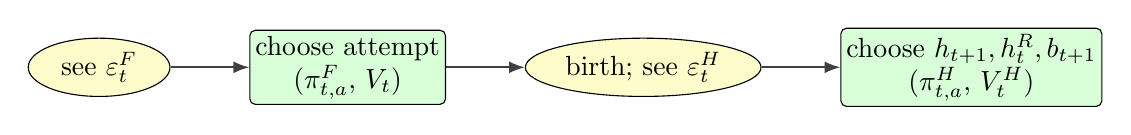
\begin{tikzpicture}[
  node distance=7mm and 10mm, >=Latex,
  see/.style={
    ellipse, draw, fill=yellow!20,
    minimum height=1.3em, minimum width=1.8cm,
    inner sep=2pt, align=center, font=\normalsize
  },
  choose/.style={
    rectangle, draw, fill=green!15, rounded corners=2pt,
    minimum height=1.5em, minimum width=1cm,
    inner sep=2pt, align=center, font=\normalsize
  },
  line/.style={-Latex, semithick, draw=black!75}
]
\node (fertS) [see,    alt=<3>{draw=red, ultra thick}{}] {see $\varepsilon_t^F$};
\node (fertD) [choose, right=of fertS, alt=<3>{draw=red, ultra thick}{}] {choose attempt\\($\pi^F_{t,a}$, $V_t$)};
\node (locS)  [see,    right=of fertD, alt=<3>{draw=red, ultra thick}{}] {birth; see $\varepsilon_t^H$};
\node (locD)  [choose, right=of locS,  alt=<2-3>{draw=red, ultra thick}{}] {choose $h_{t+1},h_t^R,b_{t+1}$\\($\pi^H_{t,a}$, $V^H_t$)};

\draw[line] (fertS) -- (fertD);
\draw[line] (fertD) -- (locS);
\draw[line] (locS)  -- (locD);
\end{tikzpicture}%
}

\par\vspace{0.35em}
\raggedright
}
\only<2-3>{%
\centering
\scalebox{0.85}{%
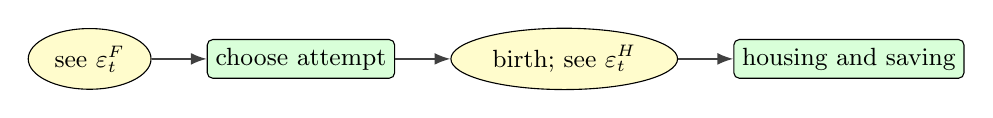
\begin{tikzpicture}[
  node distance=7mm and 7mm, >=Latex,
  see/.style={ellipse, draw, fill=yellow!20, inner sep=3pt, align=center, font=\small},
  choose/.style={rectangle, draw, fill=green!15, rounded corners=2pt, inner sep=3pt, align=center, font=\small},
  line/.style={-Latex, semithick, draw=black!75}
]
\node (fertS) [see, alt=<3>{draw=red, ultra thick}{}] {see $\varepsilon_t^F$};
\node (fertD) [choose, right=of fertS, alt=<3>{draw=red, ultra thick}{}] {choose attempt};
\node (succ) [see, right=of fertD, alt=<2>{draw=red, ultra thick}{}] {birth; see $\varepsilon_t^H$};
\node (house) [choose, right=of succ, alt=<2>{draw=red, ultra thick}{}] {housing and saving};
\draw[line] (fertS) -- (fertD);
\draw[line] (fertD) -- (succ);
\draw[line] (succ) -- (house);
\end{tikzpicture}%
}
\par\vspace{0.3em}
\raggedright
\small
\setlength{\abovedisplayskip}{4pt}\setlength{\belowdisplayskip}{4pt}

}
\raggedright
\small
\setlength{\abovedisplayskip}{4pt}\setlength{\belowdisplayskip}{4pt}

\only<1>{%
\small
\setlength{\abovedisplayskip}{6pt}\setlength{\belowdisplayskip}{6pt}

\textbf{State.}
\[
(b_t,h_t,z_t,a,n_t,m_t), \qquad h_t \in \{0,H_1,\dots,H_K\}.
\]

\begin{itemize}\setlength\itemsep{3pt}
  \item $b_t$: liquid wealth; $h_t$: owner-occupied size ($h_t=0$ if renter); $z_t$: earnings; $a$: age.
  \item $n_t$: fertility; $m_t$: children at home.
  \item After the birth outcome, $\widetilde n_t$ is the period's fertility state; if no birth, $\widetilde n_t=n_t$.
\end{itemize}

\medskip
\textbf{Within the period:} choose whether to attempt a birth, then $(h_{t+1},h_t^R,b_{t+1})$.\\[2pt]
A renter sets $h_{t+1}=0$; an owner sets $h_t^R=0$.
}

\only<2>{%
\textbf{Conditional on the realized family size:}
\[
\begin{aligned}
&V^H_t(b_t,h_t,z_t,a,\widetilde n_t,\widetilde m_t)\\
&=\E_{\varepsilon_t^H}\max_{h_{t+1},h_t^R,b_{t+1}}\Bigl\{
 u_t(c_t,s_t;\widetilde m_t)+\varepsilon_t^H(h_{t+1})\\
&\qquad+\beta\E_t\!\left[s_a V_{t+1}(b_{t+1},h_{t+1},z_{t+1},a+1,n_{t+1},m_{t+1})\right]\\
&\qquad+\beta\E_t\!\left[(1-s_a)B(w^e_{t+1})\right]\Bigr\}.
\end{aligned}
\]
\begin{itemize}\setlength\itemsep{0.5em}
 \item Total births carry forward: $n_{t+1}=\widetilde n_t$. Earnings and child maturation determine $z_{t+1}$ and $m_{t+1}$.
 \item A renter sets $h_{t+1}=0$; an owner sets $h_t^R=0$. The budget determines $c_t$.
\end{itemize}
}

\only<3>{%
At $(b_t,h_t,z_t,a,n_t,m_t)$, waiting and attempting have values
\[
\begin{aligned}
W_t^0&=V^H_t(b_t,h_t,z_t,a,n_t,m_t),\\
W_t^A&=\pi_a\!\left[V^H_t(b_t,h_t,z_t,a,n_t+1,m_t+1)-F_1\1\{n_t=0\}\right]\\
&\quad +(1-\pi_a)V^H_t(b_t,h_t,z_t,a,n_t,m_t).
\end{aligned}
\]
Before fertility tastes, household value is
\[
V_t(b_t,h_t,z_t,a,n_t,m_t)
=\E_{\varepsilon_t^F}\max\{W_t^0+\varepsilon_{t,0}^F,\ W_t^A+\varepsilon_{t,A}^F\}.
\]
The probability of attempting is
\[
\pi^F_{t,a}(b_t,h_t,z_t,n_t,m_t)
=\frac{\exp\{W_t^A/\kappa(n_t)\}}
{\exp\{W_t^A/\kappa(n_t)\}+\exp\{W_t^0/\kappa(n_t)\}},
\]
Here $\kappa(n_t)=\kappa_1$ if $n_t=0$ and $\kappa_C$ otherwise. Expected births equal $\pi_a\pi^F_{t,a}$; attempts require fertile age and family size below the maximum.
}
\end{frame}

\begin{frame}{Population and Households}
Births change future housing demand by changing the number and age of households.

\medskip
\begin{itemize}\setlength\itemsep{0.65em}
  \item $N_t=N_{t,0}$: resident persons at the start of period $t$, tracked by age and sex.
  \item $H_t$: household heads, obtained from persons using age--sex headship rates.
  \item $G_t$: the distribution of household wealth, earnings, tenure, and children.
\end{itemize}

\medskip
Births enter the population immediately. Survival, migration, and household formation determine when they add to housing demand.

\vfill
\hfill\hyperlink{person-accounting}{\beamergotobutton{Population accounting}}
\end{frame}

\begin{frame}{Equilibrium}
\small
An equilibrium is a sequence of policy functions, value functions, household distributions, populations, prices, transfers, and pensions such that:
\begin{enumerate}\setlength\itemsep{0pt}
  \item Given prices, fiscal paths, and expectations, policies solve the household's problem and values give the associated lifetime utilities.
  \item Within period $t$, annual steps $j$ and fixed headship rates satisfy:
  \[
  \begin{gathered}
  N_{t,j+1}=A_{t,j+1}N_{t,j}+f_{t,j+1}B_{t,j+1}+M_{t,j+1},\\
  H_{t,j}^{g,\ell}=\rho^{g,\ell}N_{t,j}^{g,\ell},\qquad N_{t+1,0}=N_{t,L}.
  \end{gathered}
  \]
  Fertility determines $B$; $A$ ages survivors, $fB$ counts newborn survivors, and $M$ is net migration. $L$ counts annual steps; $\ell$ is age in years.
  \item From the initial state, distributions follow policies, idiosyncratic shocks, and demographic entry and exit, with $\int dG_t=H_t$, the head count over represented adult ages.
  \item Housing clears, $\int q_t\,dG_t=H_t^s$, with $q_t$ measured in physical rooms. Asset pricing and the pay-as-you-go pension rule hold.
\end{enumerate}
\end{frame}

\section{Empirics}

\begin{frame}[plain,c,noframenumbering]{}
\centering
{\Large\textbf{Empirics}}
\end{frame}

\begin{frame}{Data}
\begin{itemize}\setlength\itemsep{0.75em}
 \item \textbf{AHS and ACS:} housing sizes, tenure, household composition, and age profiles.
 \item \textbf{PSID:} housing around childbirth, earnings, and wealth by age.
 \item \textbf{CPS and natality records:} completed fertility, childlessness, and birth timing.
 \item \textbf{Census population estimates:} age--sex population and demographic flows.
\end{itemize}

\vfill
Cross-sectional housing patterns discipline access to space; longitudinal data describe housing adjustment around births.
\end{frame}

\begin{frame}{Big Units Are Owned}
\centering
\includegraphics[width=0.77\textwidth,height=0.77\textheight,keepaspectratio]{../code/data/ahs_supply_snapshot/output_ahs_family_unit_menu_national/ahs_tenure_share_within_size.png}
\source{American Housing Survey, 2023.}
\end{frame}

\begin{frame}{Ownership and Housing Size Around First Birth}
\begin{columns}[T]
\begin{column}{0.48\textwidth}
\centering
{\small Ownership probability}

\smallskip
\includegraphics[width=\linewidth]{../../Outputs/Graphs/own_f_c_y_all.png}
\end{column}
\begin{column}{0.48\textwidth}
\centering
{\small Number of rooms}

\smallskip
\includegraphics[width=\linewidth]{../../Outputs/Graphs/rooms_f_c_y_all.png}
\end{column}
\end{columns}

\medskip
\small Original May event-study coefficients; measurement revisions under review.
\source{PSID; original May event-study estimates.}
\end{frame}

\begin{frame}{Moving Around First Birth}
\begin{columns}[T]
\begin{column}{0.48\textwidth}
\centering
{\small Expansion or better housing}

\smallskip
\includegraphics[width=\linewidth]{../../Outputs/Graphs/mv_s_f_c_y_all.png}
\end{column}
\begin{column}{0.48\textwidth}
\centering
{\small Neighborhood, schools, or proximity}

\smallskip
\includegraphics[width=\linewidth]{../../Outputs/Graphs/mv_n_f_c_y_all.png}
\end{column}
\end{columns}

\medskip
\small Original May event-study coefficients; measurement revisions under review.
\source{PSID; original May event-study estimates.}
\end{frame}

\section{Quantification}

\begin{frame}[plain,c,noframenumbering]{}
\centering
{\Large\textbf{Quantification}}
\end{frame}


% Initial tables and fit coordinates: verified_final/selected_target_fit.csv and selected_parameters.csv (2026-09-12).
% Fingerprint c0e266d3a0d430343c469d780d1aedb45fa87f8763c9c938889e0c37daa31de2.

\begin{frame}{Calibration and Historical Transition}
\begin{enumerate}\setlength\itemsep{1.1em}
  \item \textbf{Calibrate the 2007 steady state.}\\
  Match fertility, housing, and wealth moments to determine household parameters.
  \item \textbf{Estimate the sequence of fertility shocks.}\\
  Hold those parameters fixed and match birth rates through 2023 with unanticipated changes in fertility preferences. Carry households and population forward between shocks.
  \item \textbf{Project the economy forward.}\\
  After 2023, hold fertility preferences fixed and solve for prices, housing choices, and population. Compare housing policies from the same 2023 economy.
\end{enumerate}
\end{frame}


\begin{frame}{Historical Fertility Discipline}
\small
Choose each preference level to match fertility over the following four calendar years.

\medskip
\renewcommand{\arraystretch}{1.15}
\begin{tabularx}{\textwidth}{@{}C C C@{}}
\toprule
Decision date & Birth years & Mean published TFR \\
\midrule
2007 & 2008--2011 & 1.9749 \\
2011 & 2012--2015 & 1.8610 \\
2015 & 2016--2019 & 1.7554 \\
2019 & 2020--2023 & 1.6458 \\
\bottomrule
\end{tabularx}

\medskip
The model sums age-specific births per adult household: an approximate analogue of female period TFR. The exposure mapping remains to be reconciled.

\medskip
This is the estimation design. A complete historical fit requires converged conditional equilibria and stability to a longer continuation horizon.
\source{Published annual U.S. total fertility rates; equal-weight four-year averages.}
\end{frame}



\begin{frame}{Empirical Discipline}
\small
Moments inform parameters through their joint effects on household choices.

\medskip
\renewcommand{\arraystretch}{1.22}
\begin{tabularx}{\textwidth}{@{}>{\raggedright\arraybackslash}p{0.14\textwidth}Y>{\raggedright\arraybackslash}p{0.19\textwidth}@{}}
\toprule
Margin & Empirical variation & Parameters \\
\midrule
Fertility & Childlessness and one-child families; mean first-birth age and the share at age 30+ & $F_1,\kappa_1,\kappa_C$ \\
Housing & Rooms and ownership; housing around first birth and differences across family sizes & $h_P,\chi,H_0$ \\
Saving & Wealth relative to earnings, bequest flows, and old-age wealth dispersion & $\beta,\theta_0,\theta_1$ \\
\bottomrule
\end{tabularx}

\medskip
Fertility stocks and birth timing discipline different margins. Housing around birth informs demand for space.
\end{frame}

\begin{frame}{Moment Construction}
\small
Compare model moments with the same age windows, conditioning events, and time units used in the data.

\medskip
\begin{itemize}\setlength\itemsep{0.65em}
 \item \textbf{Fertility:} CPS 2004/2006 children ever born at ages 40--44; natality records 2003--2006 for first-birth timing. Interpolate birth timing within model age cells.
 \item \textbf{Housing:} ACS 2005/2006, pooled across 42 metros; match room top-codes, age ranges, and resident-child groups. The model uses dependent counts as the child-group proxy.
 \item \textbf{Wealth:} PSID 2003/2005; match weighted wealth/earnings and old-age wealth/income dispersion. Bequests/wealth is an external flow restriction.
 \item \textbf{Housing around birth:} compare a longitudinal PSID room response with the corresponding model event contrast; the empirical timing and reference design remain under review.
\end{itemize}
\end{frame}

\begin{frame}{Calibration: Targets and Model}
\footnotesize
\linespread{1}\selectfont
\renewcommand{\arraystretch}{1.12}
\begin{tabularx}{\textwidth}{@{}Xrr@{}}
\toprule
Moment & Target & Model \\
\midrule
Completed fertility (normalization) & 2.10 & 2.10 \\
Childless, women 40--44 (\%) & 19.8 & 20.7 \\
Exactly one child among mothers, 40--44 (\%) & 21.4 & 20.7 \\
Mean age at first birth (years) & 25.98 & 26.10 \\
First births at age 30+ (\%) & 24.9 & 23.2 \\
\addlinespace[4pt]
Mean occupied rooms (capped at 9) & 5.56 & 6.29 \\
Ownership, heads 30--55 (\%) & 64.8 & 52.4 \\
First-birth room response, $-1$ to $+3$ & 0.720 & 1.011 \\
Rooms: 3+ versus 1--2 resident children & 0.347 & 0.200 \\
Recent-parent ownership gap (pp) & 16.3 & 15.0 \\
\addlinespace[4pt]
Wealth / annual gross earnings & 6.15 & 4.85 \\
Annual bequests / wealth (\%) & 0.88 & 0.86 \\
Wealth/income p90 / median, ages 76--84 & 3.52 & 4.44 \\
\bottomrule
\end{tabularx}
\end{frame}
\begin{frame}{Calibrated Parameters}
\footnotesize

\renewcommand{\arraystretch}{1.12}
\begin{tabularx}{\textwidth}{@{}lXr@{}}
\toprule
Parameter & Economic interpretation & Value \\
\midrule
$\beta_{\rm annual}$ & Annual discount factor & 0.990 \\
$\kappa_1$ & First-birth taste dispersion & 0.279 \\
$\kappa_C$ & Later-birth taste dispersion & 0.347 \\
$\chi$ & Owner housing-service multiplier & 1.048 \\
$H_0$ & Housing supply at reference price & 8.191 \\
$\theta_0$ & Bequest-motive scale & 0.087 \\
$\theta_1$ & Bequest-utility wealth shift & 0.057 \\
$F_1$ & First-birth utility cost & 0.127 \\
$h_P$ & Parenthood space requirement & 2.300 \\

\bottomrule
\end{tabularx}\par
\medskip
$\beta_{\rm annual}$ and $h_P$ reach their upper search bounds.
\hfill\hyperlink{parameter-restrictions}{\beamergotobutton{Parameter restrictions}}
\end{frame}

\begin{frame}{External Inputs and Normalizations}
\footnotesize
\renewcommand{\arraystretch}{1.18}
\begin{tabularx}{\textwidth}{@{}>{\raggedright\arraybackslash}p{0.34\textwidth}>{\raggedright\arraybackslash}p{0.25\textwidth}>{\raggedright\arraybackslash}X@{}}
\toprule
Parameter & Value & Source \\
\midrule
Risk aversion $\sigma$ & 2 & \\
Equivalence scale $e(\widetilde m_t)$ & $\bigl((2+0.7\widetilde m_t)/2\bigr)^{0.7}$ & Scholz, Seshadri \& Khitatrakun (2006) \\
Consumption share $\alpha_0$ & 0.733 & CEX childless cash renters, 2019--2023 \\
Housing-supply elasticity $\eta$ & 0.63 & \\
Housing-taste dispersion $\kappa_H$ & 0.005 & \\
Annual real return $i_{\mathrm{ann}}$ & 2.0\% & Greaney et al.\ (2025) \\
Payroll tax rate $\tau^{SS}$ & 17.9\% & OECD U.S. average \\
Initial fertility preference $\psi_0$ & 0.1596 & Completed fertility of 2.1 \\
\bottomrule
\end{tabularx}\par
\medskip
A model period contains $L=4$ calendar years, $\beta=\beta_{\rm annual}^4$.
\end{frame}

% Checked presentation patch: stationary household fits through 2019,
% then the actual dated forward forecast from source PATCH17497354_0.
\begin{frame}{Historical Fertility}
\centering
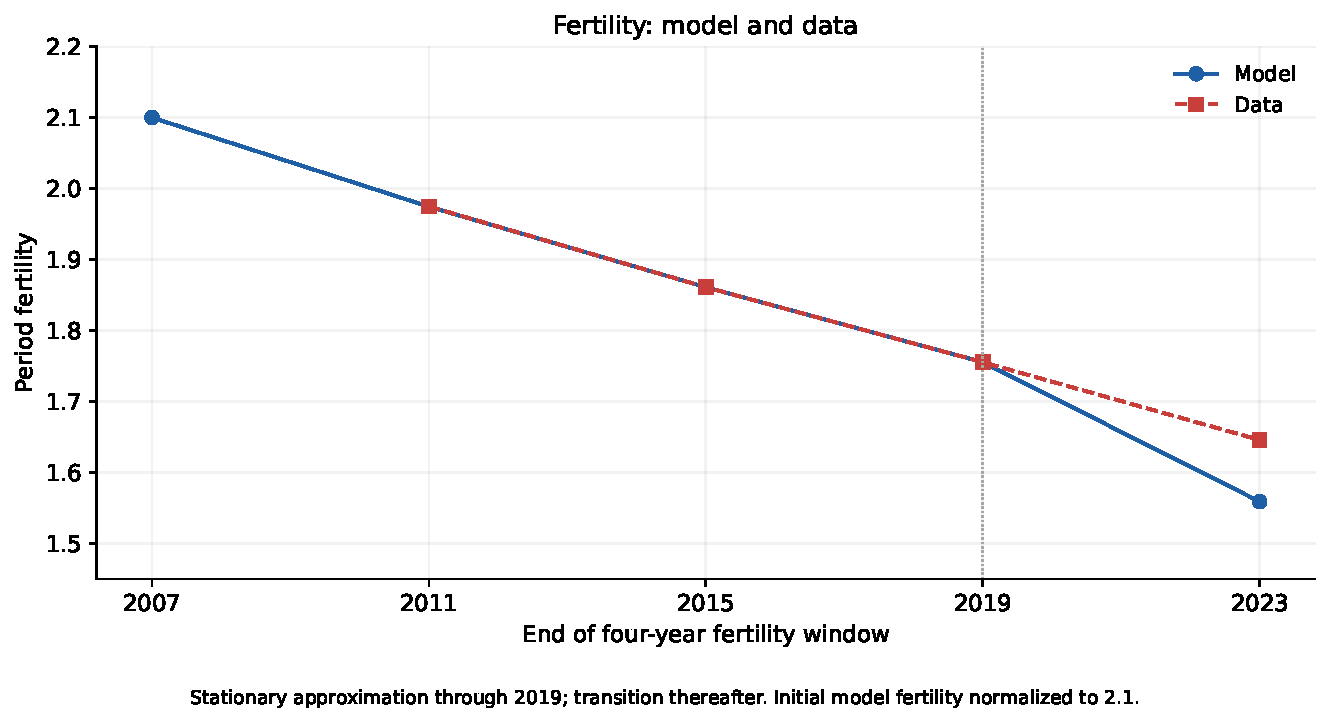
\includegraphics[width=\textwidth,height=0.78\textheight,keepaspectratio]{../output/model/e5f_matched_pf_20260909a/current_candidate_transition/overnight_20260912/patch_readout/figures/historical_fertility.pdf}
\par\smallskip
\scriptsize The final fertility window is not yet matched; the terminal horizon is not verified.
\end{frame}

\begin{frame}{The 2023 Equilibrium}
\centering
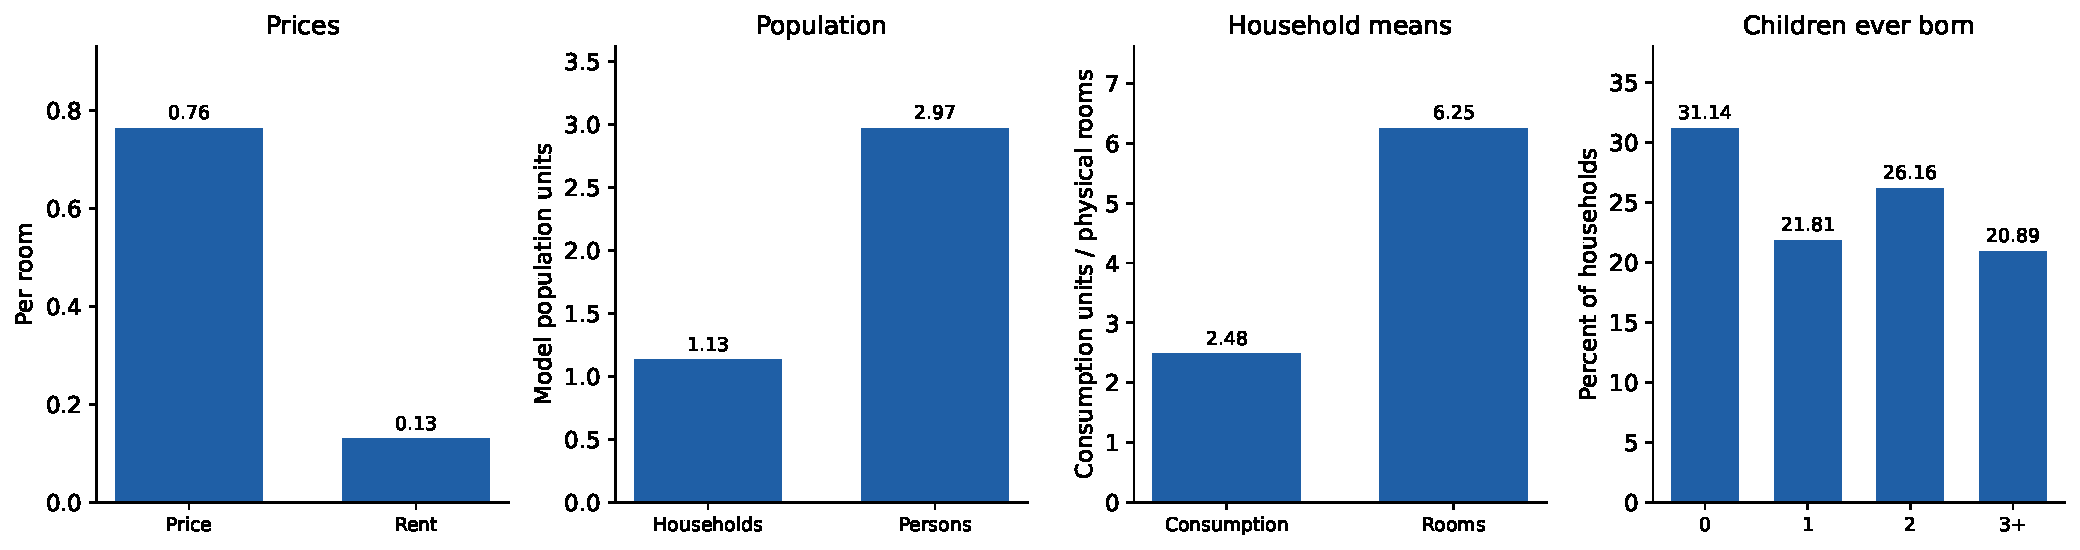
\includegraphics[width=\textwidth,height=0.85\textheight,keepaspectratio]{../output/model/e5f_matched_pf_20260909a/current_candidate_transition/overnight_20260912/patch_readout/figures/equilibrium_2023.pdf}
\par\smallskip
\scriptsize Population levels and age composition are externally conditioned.
\end{frame}

\begin{frame}{Lifecycle Fit in 2023}
\centering
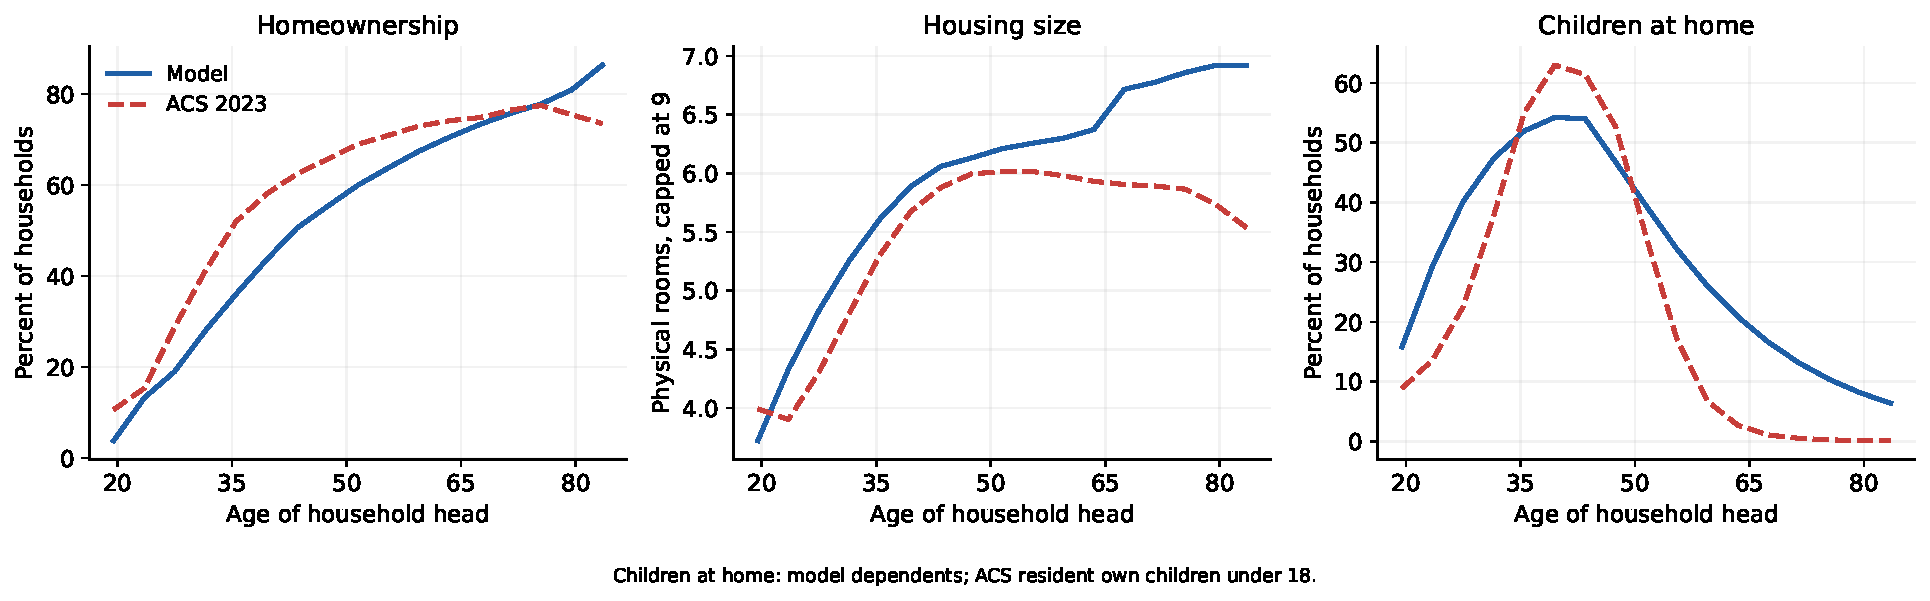
\includegraphics[width=\textwidth,height=0.85\textheight,keepaspectratio]{../output/model/e5f_matched_pf_20260909a/current_candidate_transition/overnight_20260912/patch_readout/figures/lifecycle_2023.pdf}
\par\smallskip
\scriptsize 2023 profiles are untargeted comparisons; the calibration uses initial-period moments.
\end{frame}

\begin{frame}{Intergenerational Allocation: Model vs Data}
\centering
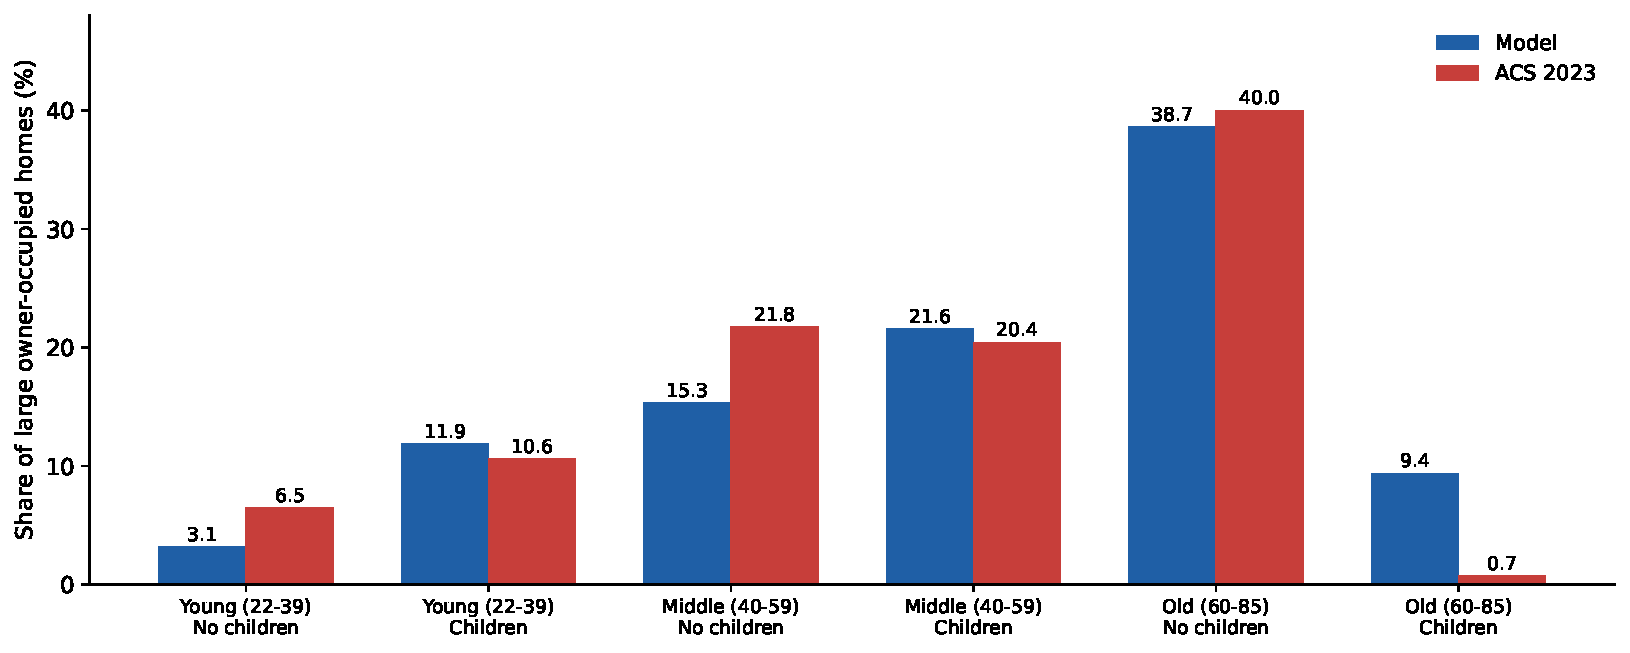
\includegraphics[width=0.92\linewidth,height=0.78\textheight,keepaspectratio]{../output/model/e5f_matched_pf_20260909a/current_candidate_transition/overnight_20260912/patch_readout/figures/intergenerational_allocation_2023.pdf}
\par\smallskip
\scriptsize Owner-occupied homes with $6+$ rooms; ACS 2023. Children: model dependents; ACS resident own minors.
\end{frame}

\begin{frame}{Housing and Fertility in Equilibrium}
The next three diagrams illustrate the interaction between housing costs and population.

\medskip
\begin{itemize}\setlength\itemsep{0.65em}
 \item \textbf{Left panel:} $P(S;v)$ is the housing cost that clears the market at adult-household population $S$, holding age composition fixed.
 \item \textbf{Right panel:} $n(p;v)$ is household fertility at housing cost $p$ and fertility preference $v$.
 \item The illustration uses a closed population, with replacement equal to $n=1$.
\end{itemize}

\vfill
These are schematic schedules. The quantitative model tracks the full age distribution and distinguishes rents from asset prices.
\end{frame}

\begin{frame}{Initial Steady State}
\centering
\includegraphics[width=\textwidth,height=0.66\textheight,keepaspectratio]{../output/model/fertility_population_housing_transition_note/housing_fertility_stage_initial.pdf}

\medskip
\raggedright\small
At $A$, housing clears at $(S_0,p_0)$ and fertility is at replacement.\par
The housing cost and population are constant in this schematic initial economy.
\end{frame}



\begin{frame}{Impact}
\centering
\includegraphics[width=\textwidth,height=0.60\textheight,keepaspectratio]{../output/model/fertility_population_housing_transition_note/housing_fertility_stage_impact.pdf}

\medskip
\raggedright\small
A fall from $v_0$ to $v_1$ shifts both schedules. With $S_0$ inherited, the schematic impact equilibrium moves from $A$ to $I$: housing cost and fertility fall.

\smallskip
The diagram shows a one-time shift; the quantitative preference decline is spread over time.
\end{frame}

\begin{frame}{Demographic Adjustment}
\centering
\includegraphics[width=\textwidth,height=0.60\textheight,keepaspectratio]{../output/model/fertility_population_housing_transition_note/housing_fertility_stage_adjustment.pdf}

\medskip
\raggedright\small
Smaller entering cohorts can reduce housing demand. Lower housing costs partly offset the preference decline; $A'$ marks a possible stationary outcome.

\smallskip
The arrow links the illustrated equilibria. Changing age composition can produce overshooting; it is not a computed transition or a convergence result.
\end{frame}

\begin{frame}{Housing Policy During the Transition}
We study whether a rebated property tax changes access to family housing and fertility during the demographic transition.

\medskip
\begin{itemize}\setlength\itemsep{0.8em}
 \item \textbf{Starting point:} the same inherited 2023 economy---liquid assets, homes, and age distributions.
 \item \textbf{Experiment:} a permanent increase in the annual property-tax rate from 1\% to 2\%; each path rebates its revenue equally to household heads.
 \item \textbf{Common environment:} the fertility-preference path, housing supply schedule, survival, migration, and entry rule.
\end{itemize}

\vfill
Compare the initial response of prices and household choices, then the evolution of births, population, and housing demand.
\end{frame}

\begin{frame}{The Rebated Property Tax}
\small
In each path, all property-tax revenue is returned equally to household heads:
\[
T_t\int dG_t=\tau_t^p P_t Q_t^H,
\qquad Q_t^H=\int q_t(x_t)\,dG_t(x_t).
\]
Here $q_t(x_t)$ is occupied physical housing, including rented rooms; $\tau_t^p$ is the tax rate per model period.

\begin{itemize}\setlength\itemsep{0.5em}
 \item \textbf{Housing costs:} carrying costs affect asset prices and rents.
 \item \textbf{Household resources:} rebates change disposable income and saving; prices change the required down payment.
 \item \textbf{Family choices:} tenure, housing size, and fertility respond jointly.
 \item \textbf{Demographic feedback:} births change future cohorts and housing demand.
\end{itemize}

\vfill
The payroll tax is unchanged; a separate balanced budget determines pensions in each path.
\end{frame}

\begin{frame}{Conclusion}
\begin{itemize}\setlength\itemsep{0.85em}
 \item Children raise demand for rooms; rental size and down payments govern access to that space.
 \item Tenure, saving, and fertility interact over the household lifecycle.
 \item Births change population and housing demand with long delays.
 \item Housing policy changes choices along an ongoing demographic transition.
\end{itemize}

\vfill
\textbf{The policy comparison is between paths starting from the same inherited economy.}
\end{frame}

\begin{frame}[plain,c,noframenumbering]{}
\centering{\Huge Thank You}
\end{frame}

\appendix

\begin{frame}[plain,c,noframenumbering]{}
\centering{\Large\textbf{Appendix}}
\end{frame}



\begin{frame}{1. Calibrating the Initial Economy}
\linespread{1}\fontsize{9}{11}\selectfont
\textbf{Goal:} fit pre-2007 household moments. External inputs and all 12 targets and weights stay fixed.

\medskip
\begin{enumerate}\setlength\itemsep{0.45em}
 \item \textbf{Try a parameter vector $\theta$:} nine coefficients governing saving, fertility, housing, and bequests.
 \item \textbf{Compute initial age--earnings shares} from survival, entry, and the earnings process. Set the pension to payroll revenue divided by retiree exposure; verify it against the solved distribution.
 \item \textbf{Try a fertility preference $\psi_0$ and solve the housing equilibrium.} Guess the house price $P$, derive rent, solve household choices backward, and find the stationary distribution forward. Update $P$ and repeat until housing demand equals supply.
 \item \textbf{Update $\psi_0$ with a bracketed scalar search.} Repeat step 3 for each trial until model completed fertility equals 2.1 (within 0.0005).
 \item \textbf{Score this parameter vector:} compute all 12 model moments and the weighted sum of squared model--target gaps.
 \item \textbf{Update $\theta$.} Perturb each coefficient to estimate how the moments respond; use these slopes for bounded, ridge-regularized joint steps. Redo steps 2--5 for each proposal, keep the lowest loss, and repeat within the search budget. Re-solve the selected winner twice.
\end{enumerate}

\vfill
\textbf{Nested loops:} parameter search $\longrightarrow$ fertility normalization $\longrightarrow$ housing-market clearing.
\end{frame}


\begin{frame}{2. Fitting the Historical Transition}
\linespread{1}\fontsize{9}{11}\selectfont
\textbf{Hold the nine structural parameters fixed.} Form 2007 age masses from data; within each age, keep the calibrated distribution of wealth, housing, and family states.

\medskip
\begin{enumerate}\setlength\itemsep{0.45em}
 \item \textbf{Try $\psi_{2007}$, believed permanent.} Solve the terminal stationary economy at this preference level.
 \item \textbf{Guess future price and pension paths.} Solve household choices backward from the terminal value; simulate household and person distributions and birth cohorts forward from the inherited 2007 state.
 \item \textbf{Update the price and pension paths and repeat step 2} until housing clears and the payroll budget balances at every date. Verify the population accounting, recompute the path, and check a longer horizon.
 \item \textbf{Change $\psi_{2007}$ and repeat steps 1--3} until first-window fertility matches the 2008--2011 target of 1.974875 (error at most 0.005). Every trial starts from the same 2007 state.
 \item \textbf{Advance only after acceptance.} Keep the first four-year outcome and birth queues. Repeat at 2011, 2015, and 2019 to target the following four years. Each new preference level is unanticipated.
\end{enumerate}

\medskip
After 2023, hold the final preference level fixed.
\par\smallskip
\textit{The household-rate analogue of female TFR is approximate; the complete history is not yet validated.}
\end{frame}


\begin{frame}[label=borrowing-limits]{Borrowing Limits}
\small
\setlength{\abovedisplayskip}{5pt}\setlength{\belowdisplayskip}{5pt}
After a housing transaction, liquid wealth is
\[
\widetilde b_t=b_t+\1\{h_{t+1}\neq h_t\}\bigl[(1-\psi^s)P_t h_t-P_t h_{t+1}\bigr].
\]
Let $D_{a+1}$ be the unsecured borrowing allowance and $\lambda_{a+1}$ govern repayment of inherited unsecured debt. Its lower bound is
\[
\mathcal L_{a+1}(u)=\min\{\lambda_{a+1}\min(u,0),-D_{a+1}\}.
\]
With collateral floor $C_t=-\phi P_t h_{t+1}$, saving must satisfy
\[
\begin{aligned}
\text{Renters:}\quad b_{t+1}&\geq\underline b_{t+1}^R=\mathcal L_{a+1}(\widetilde b_t),\\
\text{Owners:}\quad b_{t+1}&\geq\underline b_{t+1}^O=C_t+\mathcal L_{a+1}(\widetilde b_t-C_t).
\end{aligned}
\]
A purchase ($h_{t+1}>0$, $h_{t+1}\neq h_t$) separately requires
\[
b_t+(1-\psi^s)P_t h_t\geq(1-\phi)P_t h_{t+1}.
\]
Inherited unsecured debt can run off gradually, including for renters.
\end{frame}

\begin{frame}[label=parameter-restrictions]{Parameter Restrictions}
\footnotesize
\renewcommand{\arraystretch}{1.12}
\begin{tabularx}{\textwidth}{@{}lrrrX@{}}
\toprule
Parameter & Value & Lower & Upper & Position \\
\midrule
$\beta_{\rm annual}$ & 0.9900 & 0.94 & 0.99 & Upper bound \\
$\kappa_1$ & 0.2794 & 0.02 & 50 & Near lower bound \\
$\kappa_C$ & 0.3469 & 0.02 & 50 & Near lower bound \\
$\chi$ & 1.0480 & 0.1 & 5 & Interior \\
$H_0$ & 8.1905 & 0.2 & 80 & Interior \\
$\theta_0$ & 0.0870 & 0 & 8 & Interior \\
$\theta_1$ & 0.0571 & 0.02 & 16 & Near lower bound \\
$F_1$ & 0.1268 & 0 & 8 & Interior \\
$h_P$ & 2.3000 & 0.1 & 2.3 & Upper bound \\

\bottomrule
\end{tabularx}\par
\medskip
Near-bound means within 1\% of the allowed range; it does not establish a binding constraint. Fixed, normalized, and budget-derived objects are listed separately in the main table.
\end{frame}

\begin{frame}{Steady-State Equilibrium}
\small
A steady state is a constant allocation, population structure, and price:
\[
(N^*,H^*,G^*,\pi^*,P^*,r^*,T^*,\varpi^*).
\]
Households optimize, persons and household distributions reproduce themselves, housing clears, and the fiscal rule holds.

\medskip
\begin{itemize}\setlength\itemsep{0.65em}
 \item With no migration, births must replace deaths in a constant population.
 \item With migration, births and net inflows together offset deaths.
 \item A constant continuation value alone does not make a finite path stationary.
\end{itemize}
\end{frame}

\begin{frame}[label=person-accounting]{The Person-Cohort Law}
\small
$t$ indexes household periods; $j=0,\ldots,L$ indexes years within each period. $N_{t,j}^{g,\ell}$ counts persons of sex $g$ and age $\ell$ in years.

\medskip
For $j=0,\ldots,L-1$, the annual person law is
\[
N_{t,j+1}
=
A_{t,j+1}N_{t,j}+f_{t,j+1}B_{t,j+1}+M_{t,j+1}.
\]

\begin{itemize}\setlength\itemsep{0.5em}
  \item $A_{t,j+1}$ ages existing cohorts using destination-age survival.
  \item $f_{t,j+1}B_{t,j+1}$ allocates newborn survivors by sex at age zero.
  \item $M_{t,j+1}$ is the age--sex net-migration flow after survival.
  \item Model-period births are assigned to calendar cohorts before the annual law is iterated.
\end{itemize}

\vfill
The period boundary satisfies $N_{t+1,0}=N_{t,L}$; write $N_t=N_{t,0}$.
\end{frame}

\begin{frame}{The Household-Head Law}
\small
Annual age--sex headship rates $\rho^{g,\ell}$ map persons into the target head stock:
\[
H_{t,j+1}^{g,\ell}
=
\rho^{g,\ell}N_{t,j+1}^{g,\ell}
=
H_{t,j+1}^{\mathrm{surv},g,\ell}
+F_{t,j+1}^{g,\ell}
-D_{t,j+1}^{g,\ell}
+H_{t,j+1}^{M,g,\ell}.
\]

Aggregating annual ages $\ell$ into household age cells $a$, the household operator supplies
$\widetilde G_{t+1,a}$. Its mass is rescaled to the person-law head target:
\[
G_{t+1,a}(x_{t+1})
=
H_{t+1,a}
\frac{\widetilde G_{t+1,a}(x_{t+1})}
{\int\widetilde G_{t+1,a}(\xi)\,d\xi}.
\]

\begin{itemize}\setlength\itemsep{0.4em}
  \item $F$ and $D$ are the minimum one-way formation or dissolution flow needed to attain $\rho^{g,\ell}$.
  \item Wealth, tenure, income, and family composition are preserved within age.
  \item This is an accounting closure, not an estimated household-formation hazard.
\end{itemize}
\end{frame}

\begin{frame}{Exact Annual Person Accounting}
\small
Let $s^{g,\ell}$ be survival and $f^g$ the birth sex share. For newborns,
\[
N_{t,j+1}^{g,0}
=
s_{t,j+1}^{g,0}f_{t,j+1}^{g}B_{t,j+1}
+
M_{t,j+1}^{g,0}.
\]
For interior ages $\ell\geq1$,
\[
N_{t,j+1}^{g,\ell}
=
s_{t,j+1}^{g,\ell}N_{t,j}^{g,\ell-1}
+
M_{t,j+1}^{g,\ell}.
\]
The terminal age is top coded, so survivors from the penultimate and terminal
cells both enter the last cell. Every step satisfies
\[
\sum N_{t,j+1}
=
\sum N_{t,j}+B_{t,j+1}
-\text{newborn deaths}
-\text{existing deaths}
+\sum M_{t,j+1}.
\]
\end{frame}

\begin{frame}{The Within-Age Household Bridge}
Let $\widetilde G_{t+1,a}(x_{t+1})$ be the raw household transition within age $a$,
and let $H_{t+1,a}$ be the head mass implied by persons. Then
\[
G_{t+1,a}(x_{t+1})
=
\begin{cases}
\displaystyle
H_{t+1,a}
\frac{\widetilde G_{t+1,a}(x_{t+1})}
{\int\widetilde G_{t+1,a}(\xi)\,d\xi},
&
\int\widetilde G_{t+1,a}>0,
\\[1.2em]
H_{t+1,a}\Gamma_a(x_{t+1}),
&
\text{for an empty entrant age cell},
\end{cases}
\]
where $\Gamma_a$ is the externally specified entrant template. The operation
exposes added and removed mass separately and moves no mass across ages.

A richer model would estimate economic states for newly formed, dissolved,
and migrant heads rather than preserve the raw conditional composition.
\end{frame}

\begin{frame}{Housing-Market Clearing}
Let $q_t(x_t)$ denote the physical housing occupied after tenure choice. Market clearing requires
\[
Q_t^H=\int q_t(x_t)\,dG_t(x_t)
=H_0\left(\frac{P_t}{\bar P}\right)^\eta.
\]
For renters, $q_t=h_t^R$; for owners, $q_t=h_{t+1}$. Choice probabilities are included when aggregating.

\medskip
\begin{itemize}\setlength\itemsep{0.65em}
 \item The owner-service premium changes utility, not physical supply.
 \item Conditional renter policies enter demand only when renting is chosen.
 \item The same supply schedule applies to baseline and tax-reform paths.
\end{itemize}
\end{frame}

\begin{frame}{Perfect-Foresight Solution}
\begin{enumerate}\setlength\itemsep{0.7em}
 \item Guess the price and pension paths and compute rents from asset pricing.
 \item Solve households backward using date-specific continuation values.
 \item Advance household and population distributions from the inherited state.
 \item Update prices and pensions until housing clears and the payroll budget balances at every date.
 \item Extend the horizon and check that the measured outcomes are stable.
\end{enumerate}

\vfill
A stationary terminal value supplies a boundary condition; it does not establish stationarity of the simulated endpoint.
\end{frame}

\begin{frame}{Fertility by Age: Measurement Comparison}
\centering
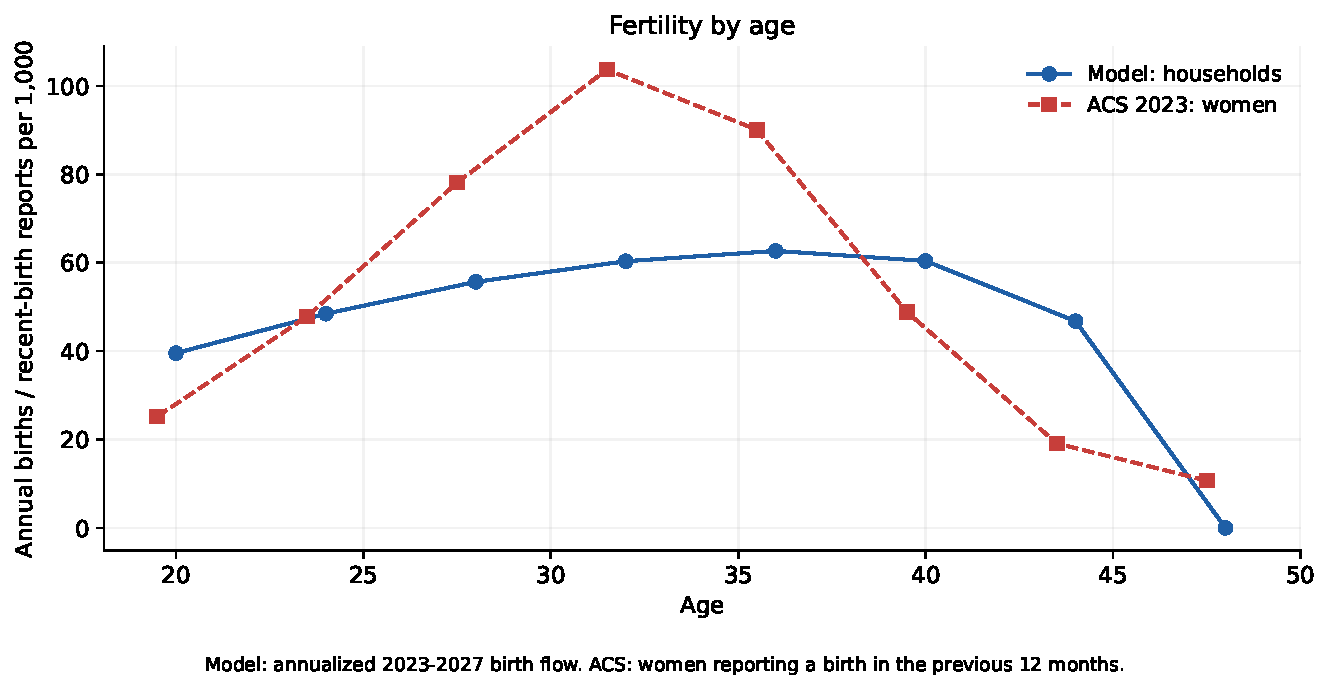
\includegraphics[width=\textwidth,height=0.85\textheight,keepaspectratio]{../output/model/e5f_matched_pf_20260909a/current_candidate_transition/overnight_20260912/patch_readout/figures/fertility_age_2023.pdf}
\end{frame}

\begin{frame}{Prices and Quantities Along the Finite Path}
\centering
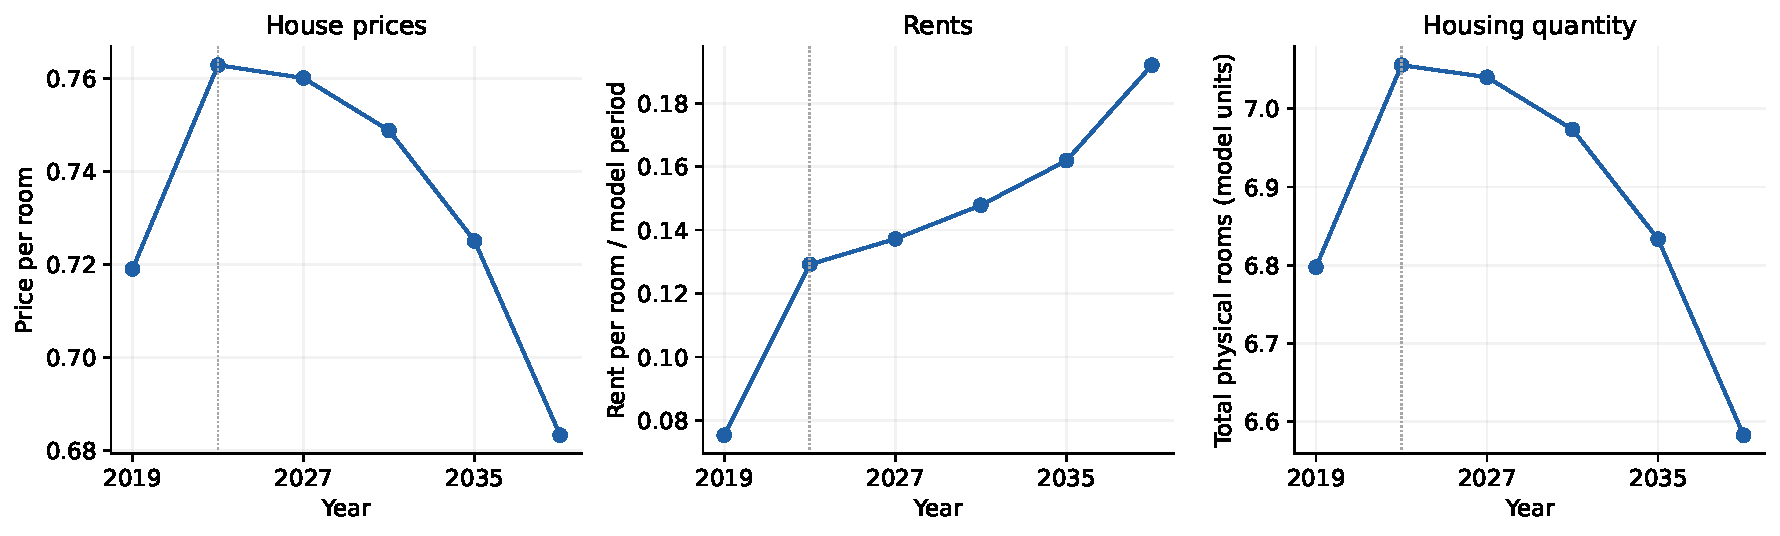
\includegraphics[width=\textwidth,height=0.85\textheight,keepaspectratio]{../output/model/e5f_matched_pf_20260909a/current_candidate_transition/overnight_20260912/patch_readout/figures/prices_quantities_path.pdf}
\end{frame}

\end{document}
